% https://tex.stackexchange.com/questions/149602/drawing-flow-diagram-in-latex-using-tikz
\documentclass[border=10pt]{standalone}
\usepackage{tikz}
\usetikzlibrary{arrows,positioning,shapes.geometric}

\begin{document}
    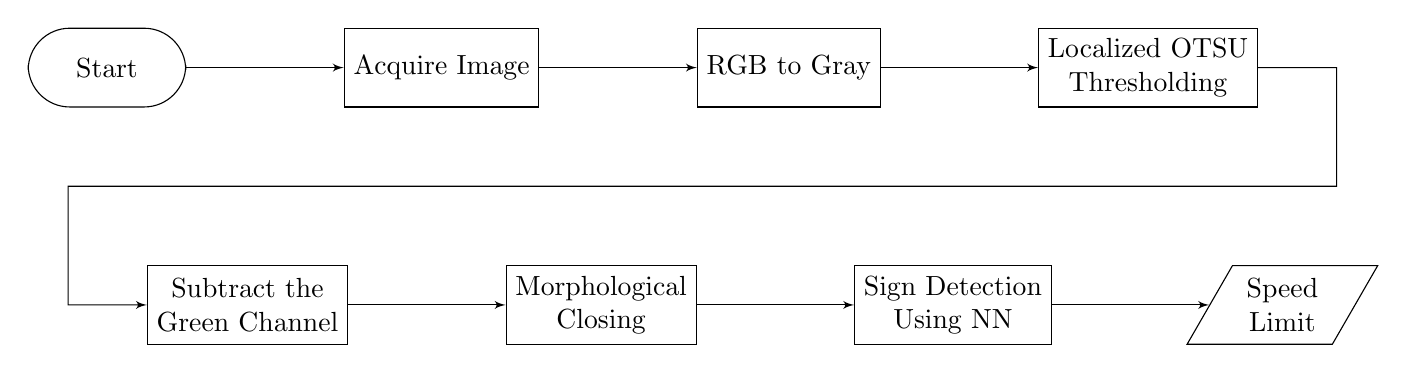
\begin{tikzpicture}[>=latex']
        \tikzset{block/.style= {draw, rectangle, align=center,minimum width=2cm,minimum height=1cm},
        rblock/.style={draw, shape=rectangle,rounded corners=1.5em,align=center,minimum width=2cm,minimum height=1cm},
        input/.style={ % requires library shapes.geometric
        draw,
        trapezium,
        trapezium left angle=60,
        trapezium right angle=120,
        minimum width=2cm,
        align=center,
        minimum height=1cm
    },
        }
        \node [rblock]  (start) {Start};
        \node [block, right =2cm of start] (acquire) {Acquire Image};
        \node [block, right =2cm of acquire] (rgb2gray) {RGB to Gray};
        \node [block, right =2cm of rgb2gray] (otsu) {Localized OTSU \\ Thresholding};
        \node [block, below right =2cm and -0.5cm of start] (gchannel) {Subtract the \\ Green Channel};
        \node [block, right =2cm of gchannel] (closing) {Morphological \\ Closing};
        \node [block, right =2cm of closing] (NN) {Sign Detection \\ Using NN};
        \node [input, right =2cm of NN] (limit) {Speed \\ Limit};
        \node [coordinate, below right =1cm and 1cm of otsu] (right) {};  %% Coordinate on right and middle
        \node [coordinate,above left =1cm and 1cm of gchannel] (left) {};  %% Coordinate on left and middle

%% paths
        \path[draw,->] (start) edge (acquire)
                    (acquire) edge (rgb2gray)
                    (rgb2gray) edge (otsu)
                    (otsu.east) -| (right) -- (left) |- (gchannel)
                    (gchannel) edge (closing)
                    (closing) edge (NN)
                    (NN) edge (limit)
                    ;
    \end{tikzpicture}
\end{document}